\section*{問題}

\begin{quotation}
 「今、半円ノ内ニ、図ノ\ruby{如}{ごと}キ\ruby{勾股形}{こうこけい}(直角三
 角形)ト二円アリ・・・」

 半円に直角三角形を内接させ、この直角三角形の内接円と、弓形内に
 えがいた最大の円があいひとしいときの外接円と小円の関係を問う。
\end{quotation}

\begin{center}
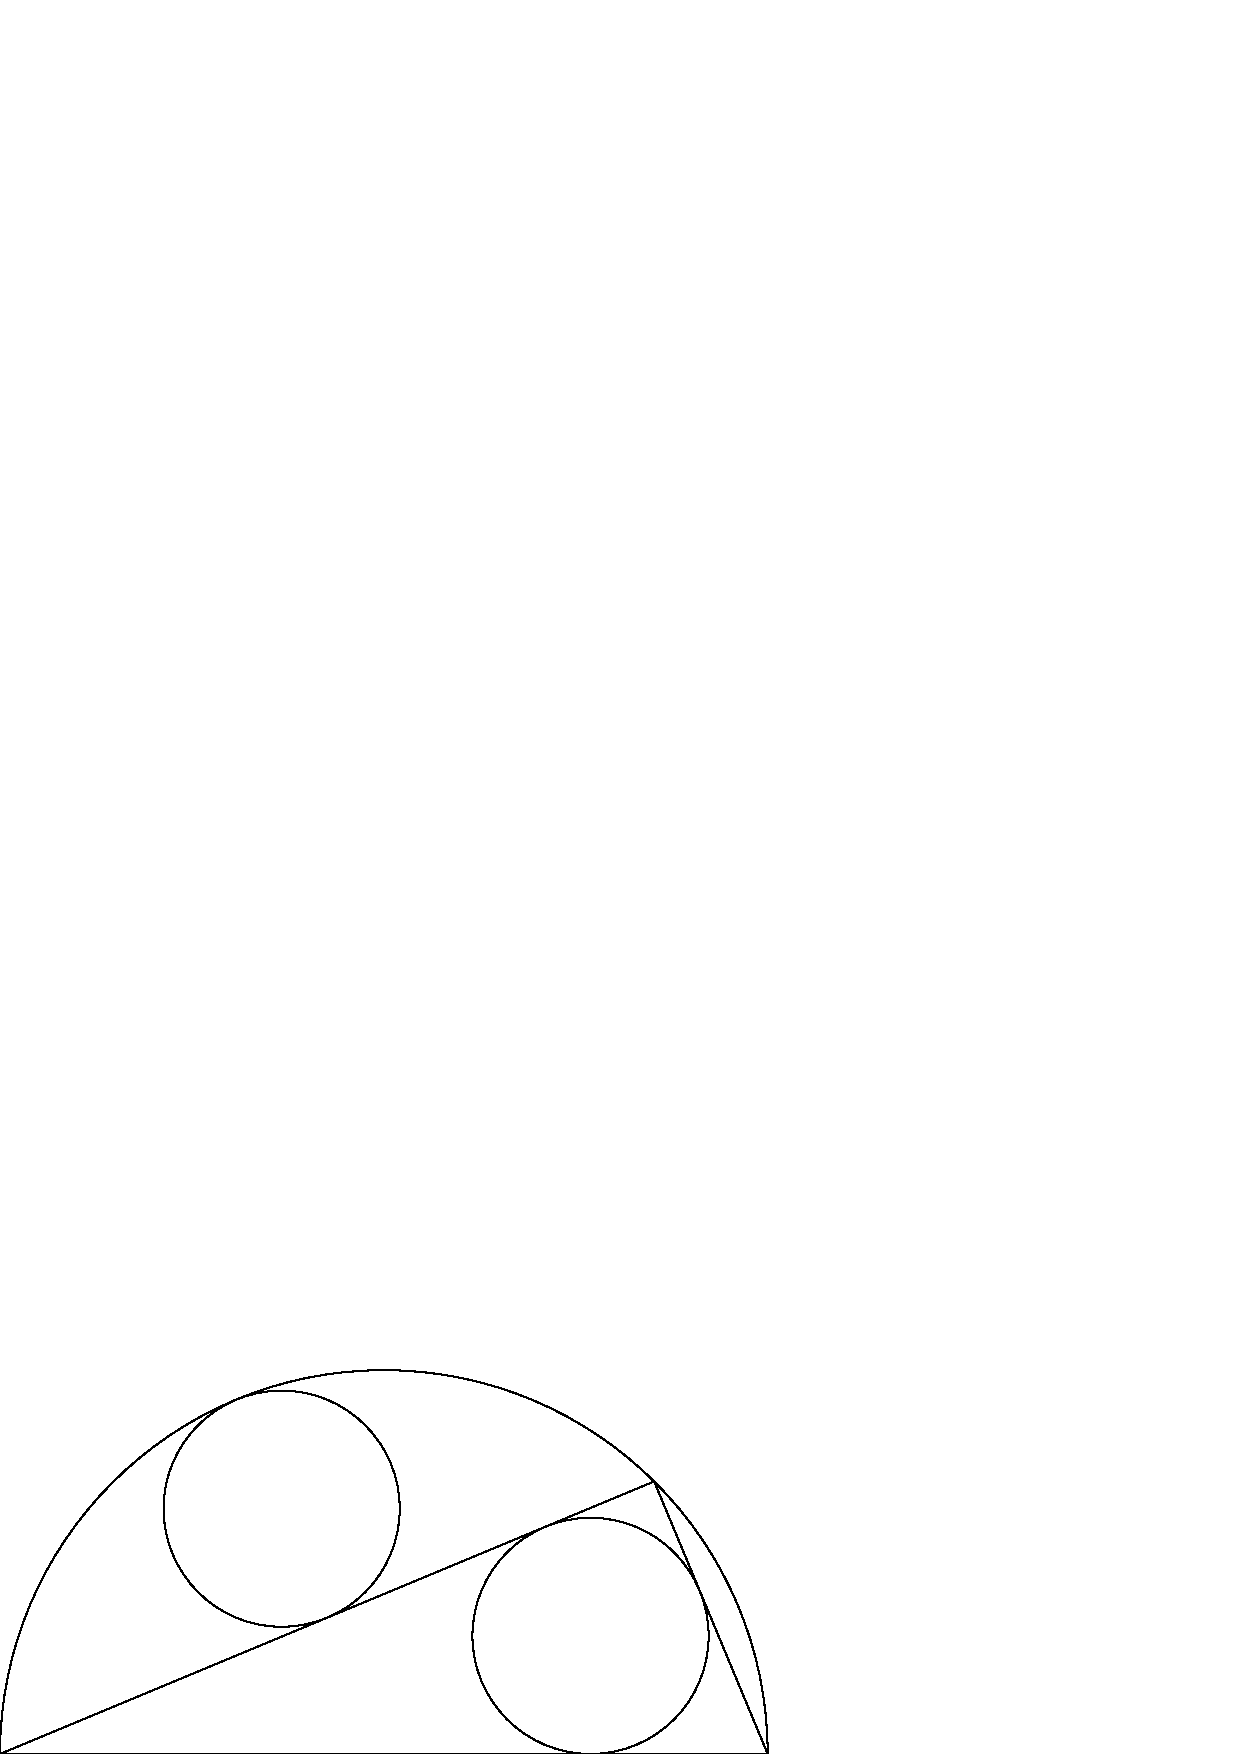
\includegraphics[height=8cm]{q1_0.pdf}
\end{center}
